\documentclass{article}
\usepackage[utf8]{inputenc}
\usepackage[margin=1in]{geometry}

\title{454 - Homework 9}
\author{Victor Zhang}
\date{November 18, 2021}

\usepackage[utf8]{inputenc}
\usepackage{amsmath}
\usepackage{amsfonts}
\usepackage{natbib}
\usepackage{graphicx}
% \usepackage{changepage}
\usepackage{amssymb}
\usepackage{xfrac}
% \usepackage{bm}
% \usepackage{empheq}
\usepackage{tikz}

\newcommand{\contra}{\raisebox{\depth}{\#}}

\newenvironment{myindentpar}[1]
  {\begin{list}{}
          {
            \setlength{\leftmargin}{#1}
            \setlength{\rightmargin}{#1}
          }
          \item[]
  }
  {\end{list}}

\pagestyle{empty}

\begin{document}

\maketitle
% \begin{center}
% {\huge Econ 482 \hspace{0.5cm} HW 3}\
% {\Large \textbf{Victor Zhang}}\
% {\Large February 18, 2020}
% \end{center}

\section*{13.5}
Suppose a digraph has no cycles. Then we may impose a topological sort on its vertices and generate a natural numbering that satisfies the conditions. Conversely, if we have a valid numbering, there are no cycles. Indeed any cycle $v_1, v_2, \dots, v_n, v_1$ must have $v_1 < v_2 < \dots < v_n$, in which case the arc $(v_n, v_1)$ would be incorrectly oriented, a contradiction $\contra$

\section*{13.6}
WLOG number the vertices $1,2,\dots, n$. By strong connection, there exists a walk from 1 to 2, 2 to 3, and so on. Most importantly, there is a walk from $n$ to 1. To create the desired closed walk just concatenate these walks.\\
Now suppose such a closed walk exists. Then the digraph must be strongly connected, since we may just follow this loop to get from any vertex $i$ to any other $j$ $\Box$

\section*{13.11}
We prove by construction. Start with an undirected graph and pick an arbitrary (undirected) cycle. Orient the edges in this cycle s.t. it is a strongly connected component. Repeat until there are no more cycles. Then the resulting (undirected) graph is a spanning forest, WLOG a spanning tree. Orient the edges greedily, starting from the root.\\
Orienting a cycle in the manner we indicate (a directed loop) maintains $indeg(v) = outdeg(v)$ for all vertices in the cycle. Since $indeg, outdeg$ are linear in the edges of the graph, orienting the edges of a spanning forest is analagous to independently orienting multiple spanning trees. Note the orientation of a subtree is independent of any sibling subtrees. Thus a greedy algorithm will always correctly maintain $|indeg(v) - outdeg(v)| \leq 1$ if we alternate in and out for the child edges of each (sub)tree root $\Box$

\section*{13.24}
The flow of each edge is marked next to the edge. Edges in the cut are marked with double lines.
\begin{figure*}[ht]
\tikzset{every picture/.style={line width=0.75pt}} %set default line width to 0.75pt        
\centering
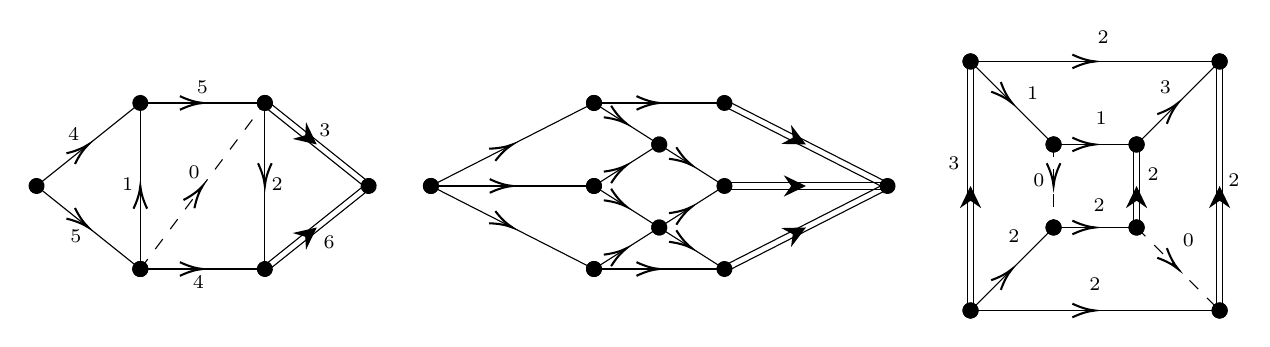
\begin{tikzpicture}[x=0.75pt,y=0.75pt,yscale=-1,xscale=1]
%uncomment if require: \path (0,341); %set diagram left start at 0, and has height of 341

%Straight Lines [id:da41597665367343417] 
\draw    (50,100) -- (100,60) ;
\draw [shift={(75,80)}, rotate = 501.34] [color={rgb, 255:red, 0; green, 0; blue, 0 }  ][line width=0.75]    (10.93,-3.29) .. controls (6.95,-1.4) and (3.31,-0.3) .. (0,0) .. controls (3.31,0.3) and (6.95,1.4) .. (10.93,3.29)   ;
\draw [shift={(50,100)}, rotate = 321.34] [color={rgb, 255:red, 0; green, 0; blue, 0 }  ][fill={rgb, 255:red, 0; green, 0; blue, 0 }  ][line width=0.75]      (0, 0) circle [x radius= 3.35, y radius= 3.35]   ;
%Straight Lines [id:da37344500106137457] 
\draw    (50,100) -- (100,140) ;
\draw [shift={(75,120)}, rotate = 218.66] [color={rgb, 255:red, 0; green, 0; blue, 0 }  ][line width=0.75]    (10.93,-3.29) .. controls (6.95,-1.4) and (3.31,-0.3) .. (0,0) .. controls (3.31,0.3) and (6.95,1.4) .. (10.93,3.29)   ;
%Straight Lines [id:da38703951681058535] 
\draw    (100,60) -- (160,60) ;
\draw [shift={(130,60)}, rotate = 180] [color={rgb, 255:red, 0; green, 0; blue, 0 }  ][line width=0.75]    (10.93,-3.29) .. controls (6.95,-1.4) and (3.31,-0.3) .. (0,0) .. controls (3.31,0.3) and (6.95,1.4) .. (10.93,3.29)   ;
\draw [shift={(100,60)}, rotate = 0] [color={rgb, 255:red, 0; green, 0; blue, 0 }  ][fill={rgb, 255:red, 0; green, 0; blue, 0 }  ][line width=0.75]      (0, 0) circle [x radius= 3.35, y radius= 3.35]   ;
%Straight Lines [id:da9159604878204042] 
\draw    (100,140) -- (160,140) ;
\draw [shift={(130,140)}, rotate = 180] [color={rgb, 255:red, 0; green, 0; blue, 0 }  ][line width=0.75]    (10.93,-3.29) .. controls (6.95,-1.4) and (3.31,-0.3) .. (0,0) .. controls (3.31,0.3) and (6.95,1.4) .. (10.93,3.29)   ;
\draw [shift={(100,140)}, rotate = 0] [color={rgb, 255:red, 0; green, 0; blue, 0 }  ][fill={rgb, 255:red, 0; green, 0; blue, 0 }  ][line width=0.75]      (0, 0) circle [x radius= 3.35, y radius= 3.35]   ;
%Straight Lines [id:da06207241473359182] 
\draw    (100,140) -- (100,60) ;
\draw [shift={(100,100)}, rotate = 450] [color={rgb, 255:red, 0; green, 0; blue, 0 }  ][line width=0.75]    (10.93,-3.29) .. controls (6.95,-1.4) and (3.31,-0.3) .. (0,0) .. controls (3.31,0.3) and (6.95,1.4) .. (10.93,3.29)   ;
\draw [shift={(100,140)}, rotate = 270] [color={rgb, 255:red, 0; green, 0; blue, 0 }  ][fill={rgb, 255:red, 0; green, 0; blue, 0 }  ][line width=0.75]      (0, 0) circle [x radius= 3.35, y radius= 3.35]   ;
%Straight Lines [id:da06697747066671744] 
\draw  [dash pattern={on 4.5pt off 4.5pt}]  (100,140) -- (160,60) ;
\draw [shift={(130,100)}, rotate = 486.87] [color={rgb, 255:red, 0; green, 0; blue, 0 }  ][line width=0.75]    (10.93,-3.29) .. controls (6.95,-1.4) and (3.31,-0.3) .. (0,0) .. controls (3.31,0.3) and (6.95,1.4) .. (10.93,3.29)   ;
\draw [shift={(100,140)}, rotate = 306.87] [color={rgb, 255:red, 0; green, 0; blue, 0 }  ][fill={rgb, 255:red, 0; green, 0; blue, 0 }  ][line width=0.75]      (0, 0) circle [x radius= 3.35, y radius= 3.35]   ;
%Straight Lines [id:da9555777085921335] 
\draw    (160,60) -- (160,140) ;
\draw [shift={(160,100)}, rotate = 270] [color={rgb, 255:red, 0; green, 0; blue, 0 }  ][line width=0.75]    (10.93,-3.29) .. controls (6.95,-1.4) and (3.31,-0.3) .. (0,0) .. controls (3.31,0.3) and (6.95,1.4) .. (10.93,3.29)   ;
\draw [shift={(160,60)}, rotate = 90] [color={rgb, 255:red, 0; green, 0; blue, 0 }  ][fill={rgb, 255:red, 0; green, 0; blue, 0 }  ][line width=0.75]      (0, 0) circle [x radius= 3.35, y radius= 3.35]   ;
%Straight Lines [id:da4263277584253127] 
\draw    (160.94,58.83) -- (210.94,98.83)(159.06,61.17) -- (209.06,101.17) ;
\draw [shift={(210,100)}, rotate = 38.66] [color={rgb, 255:red, 0; green, 0; blue, 0 }  ][fill={rgb, 255:red, 0; green, 0; blue, 0 }  ][line width=0.75]      (0, 0) circle [x radius= 3.35, y radius= 3.35]   ;
\draw [shift={(185,80)}, rotate = 218.66] [fill={rgb, 255:red, 0; green, 0; blue, 0 }  ][line width=0.08]  [draw opacity=0] (10.72,-5.15) -- (0,0) -- (10.72,5.15) -- (7.12,0) -- cycle    ;
\draw [shift={(160,60)}, rotate = 38.66] [color={rgb, 255:red, 0; green, 0; blue, 0 }  ][fill={rgb, 255:red, 0; green, 0; blue, 0 }  ][line width=0.75]      (0, 0) circle [x radius= 3.35, y radius= 3.35]   ;
%Straight Lines [id:da2199980599378284] 
\draw    (159.06,138.83) -- (209.06,98.83)(160.94,141.17) -- (210.94,101.17) ;
\draw [shift={(185,120)}, rotate = 501.34] [fill={rgb, 255:red, 0; green, 0; blue, 0 }  ][line width=0.08]  [draw opacity=0] (10.72,-5.15) -- (0,0) -- (10.72,5.15) -- (7.12,0) -- cycle    ;
\draw [shift={(160,140)}, rotate = 321.34] [color={rgb, 255:red, 0; green, 0; blue, 0 }  ][fill={rgb, 255:red, 0; green, 0; blue, 0 }  ][line width=0.75]      (0, 0) circle [x radius= 3.35, y radius= 3.35]   ;
%Straight Lines [id:da5291784344965302] 
\draw    (240,100) -- (318.57,100) ;
\draw [shift={(279.29,100)}, rotate = 180] [color={rgb, 255:red, 0; green, 0; blue, 0 }  ][line width=0.75]    (10.93,-3.29) .. controls (6.95,-1.4) and (3.31,-0.3) .. (0,0) .. controls (3.31,0.3) and (6.95,1.4) .. (10.93,3.29)   ;
%Straight Lines [id:da7415678990491239] 
\draw    (240,100) -- (318.57,60) ;
\draw [shift={(279.29,80)}, rotate = 513.02] [color={rgb, 255:red, 0; green, 0; blue, 0 }  ][line width=0.75]    (10.93,-3.29) .. controls (6.95,-1.4) and (3.31,-0.3) .. (0,0) .. controls (3.31,0.3) and (6.95,1.4) .. (10.93,3.29)   ;
\draw [shift={(240,100)}, rotate = 333.02] [color={rgb, 255:red, 0; green, 0; blue, 0 }  ][fill={rgb, 255:red, 0; green, 0; blue, 0 }  ][line width=0.75]      (0, 0) circle [x radius= 3.35, y radius= 3.35]   ;
%Straight Lines [id:da3695779911468895] 
\draw    (240,100) -- (318.57,140) ;
\draw [shift={(279.29,120)}, rotate = 206.98] [color={rgb, 255:red, 0; green, 0; blue, 0 }  ][line width=0.75]    (10.93,-3.29) .. controls (6.95,-1.4) and (3.31,-0.3) .. (0,0) .. controls (3.31,0.3) and (6.95,1.4) .. (10.93,3.29)   ;
\draw [shift={(240,100)}, rotate = 26.98] [color={rgb, 255:red, 0; green, 0; blue, 0 }  ][fill={rgb, 255:red, 0; green, 0; blue, 0 }  ][line width=0.75]      (0, 0) circle [x radius= 3.35, y radius= 3.35]   ;
%Straight Lines [id:da7993380632656581] 
\draw    (318.57,100) -- (350,80) ;
\draw [shift={(350,80)}, rotate = 327.53] [color={rgb, 255:red, 0; green, 0; blue, 0 }  ][fill={rgb, 255:red, 0; green, 0; blue, 0 }  ][line width=0.75]      (0, 0) circle [x radius= 3.35, y radius= 3.35]   ;
\draw [shift={(334.29,90)}, rotate = 507.53] [color={rgb, 255:red, 0; green, 0; blue, 0 }  ][line width=0.75]    (10.93,-3.29) .. controls (6.95,-1.4) and (3.31,-0.3) .. (0,0) .. controls (3.31,0.3) and (6.95,1.4) .. (10.93,3.29)   ;
\draw [shift={(318.57,100)}, rotate = 327.53] [color={rgb, 255:red, 0; green, 0; blue, 0 }  ][fill={rgb, 255:red, 0; green, 0; blue, 0 }  ][line width=0.75]      (0, 0) circle [x radius= 3.35, y radius= 3.35]   ;
%Straight Lines [id:da14509299231061146] 
\draw    (318.57,100) -- (350,120) ;
\draw [shift={(334.29,110)}, rotate = 212.47] [color={rgb, 255:red, 0; green, 0; blue, 0 }  ][line width=0.75]    (10.93,-3.29) .. controls (6.95,-1.4) and (3.31,-0.3) .. (0,0) .. controls (3.31,0.3) and (6.95,1.4) .. (10.93,3.29)   ;
\draw [shift={(318.57,100)}, rotate = 32.47] [color={rgb, 255:red, 0; green, 0; blue, 0 }  ][fill={rgb, 255:red, 0; green, 0; blue, 0 }  ][line width=0.75]      (0, 0) circle [x radius= 3.35, y radius= 3.35]   ;
%Straight Lines [id:da6717909557218342] 
\draw    (318.57,140) -- (350,120) ;
\draw [shift={(334.29,130)}, rotate = 507.53] [color={rgb, 255:red, 0; green, 0; blue, 0 }  ][line width=0.75]    (10.93,-3.29) .. controls (6.95,-1.4) and (3.31,-0.3) .. (0,0) .. controls (3.31,0.3) and (6.95,1.4) .. (10.93,3.29)   ;
\draw [shift={(318.57,140)}, rotate = 327.53] [color={rgb, 255:red, 0; green, 0; blue, 0 }  ][fill={rgb, 255:red, 0; green, 0; blue, 0 }  ][line width=0.75]      (0, 0) circle [x radius= 3.35, y radius= 3.35]   ;
%Straight Lines [id:da03529093809181494] 
\draw    (318.57,60) -- (350,80) ;
\draw [shift={(334.29,70)}, rotate = 212.47] [color={rgb, 255:red, 0; green, 0; blue, 0 }  ][line width=0.75]    (10.93,-3.29) .. controls (6.95,-1.4) and (3.31,-0.3) .. (0,0) .. controls (3.31,0.3) and (6.95,1.4) .. (10.93,3.29)   ;
\draw [shift={(318.57,60)}, rotate = 32.47] [color={rgb, 255:red, 0; green, 0; blue, 0 }  ][fill={rgb, 255:red, 0; green, 0; blue, 0 }  ][line width=0.75]      (0, 0) circle [x radius= 3.35, y radius= 3.35]   ;
%Straight Lines [id:da7543143852506742] 
\draw    (350,80) -- (381.43,100) ;
\draw [shift={(365.71,90)}, rotate = 212.47] [color={rgb, 255:red, 0; green, 0; blue, 0 }  ][line width=0.75]    (10.93,-3.29) .. controls (6.95,-1.4) and (3.31,-0.3) .. (0,0) .. controls (3.31,0.3) and (6.95,1.4) .. (10.93,3.29)   ;
\draw [shift={(350,80)}, rotate = 32.47] [color={rgb, 255:red, 0; green, 0; blue, 0 }  ][fill={rgb, 255:red, 0; green, 0; blue, 0 }  ][line width=0.75]      (0, 0) circle [x radius= 3.35, y radius= 3.35]   ;
%Straight Lines [id:da6275007691463839] 
\draw    (350,120) -- (381.43,100) ;
\draw [shift={(365.71,110)}, rotate = 507.53] [color={rgb, 255:red, 0; green, 0; blue, 0 }  ][line width=0.75]    (10.93,-3.29) .. controls (6.95,-1.4) and (3.31,-0.3) .. (0,0) .. controls (3.31,0.3) and (6.95,1.4) .. (10.93,3.29)   ;
\draw [shift={(350,120)}, rotate = 327.53] [color={rgb, 255:red, 0; green, 0; blue, 0 }  ][fill={rgb, 255:red, 0; green, 0; blue, 0 }  ][line width=0.75]      (0, 0) circle [x radius= 3.35, y radius= 3.35]   ;
%Straight Lines [id:da9614500105317614] 
\draw    (350,120) -- (381.43,140) ;
\draw [shift={(365.71,130)}, rotate = 212.47] [color={rgb, 255:red, 0; green, 0; blue, 0 }  ][line width=0.75]    (10.93,-3.29) .. controls (6.95,-1.4) and (3.31,-0.3) .. (0,0) .. controls (3.31,0.3) and (6.95,1.4) .. (10.93,3.29)   ;
\draw [shift={(350,120)}, rotate = 32.47] [color={rgb, 255:red, 0; green, 0; blue, 0 }  ][fill={rgb, 255:red, 0; green, 0; blue, 0 }  ][line width=0.75]      (0, 0) circle [x radius= 3.35, y radius= 3.35]   ;
%Straight Lines [id:da5773657456443695] 
\draw    (318.57,140) -- (381.43,140) ;
\draw [shift={(350,140)}, rotate = 180] [color={rgb, 255:red, 0; green, 0; blue, 0 }  ][line width=0.75]    (10.93,-3.29) .. controls (6.95,-1.4) and (3.31,-0.3) .. (0,0) .. controls (3.31,0.3) and (6.95,1.4) .. (10.93,3.29)   ;
\draw [shift={(318.57,140)}, rotate = 0] [color={rgb, 255:red, 0; green, 0; blue, 0 }  ][fill={rgb, 255:red, 0; green, 0; blue, 0 }  ][line width=0.75]      (0, 0) circle [x radius= 3.35, y radius= 3.35]   ;
%Straight Lines [id:da44150810503487237] 
\draw    (318.57,60) -- (381.43,60) ;
\draw [shift={(350,60)}, rotate = 180] [color={rgb, 255:red, 0; green, 0; blue, 0 }  ][line width=0.75]    (10.93,-3.29) .. controls (6.95,-1.4) and (3.31,-0.3) .. (0,0) .. controls (3.31,0.3) and (6.95,1.4) .. (10.93,3.29)   ;
\draw [shift={(318.57,60)}, rotate = 0] [color={rgb, 255:red, 0; green, 0; blue, 0 }  ][fill={rgb, 255:red, 0; green, 0; blue, 0 }  ][line width=0.75]      (0, 0) circle [x radius= 3.35, y radius= 3.35]   ;
%Straight Lines [id:da441434219267951] 
\draw    (382.11,58.66) -- (460.68,98.66)(380.75,61.34) -- (459.32,101.34) ;
\draw [shift={(460,100)}, rotate = 26.98] [color={rgb, 255:red, 0; green, 0; blue, 0 }  ][fill={rgb, 255:red, 0; green, 0; blue, 0 }  ][line width=0.75]      (0, 0) circle [x radius= 3.35, y radius= 3.35]   ;
\draw [shift={(420.71,80)}, rotate = 206.98] [fill={rgb, 255:red, 0; green, 0; blue, 0 }  ][line width=0.08]  [draw opacity=0] (10.72,-5.15) -- (0,0) -- (10.72,5.15) -- (7.12,0) -- cycle    ;
\draw [shift={(381.43,60)}, rotate = 26.98] [color={rgb, 255:red, 0; green, 0; blue, 0 }  ][fill={rgb, 255:red, 0; green, 0; blue, 0 }  ][line width=0.75]      (0, 0) circle [x radius= 3.35, y radius= 3.35]   ;
%Straight Lines [id:da4050416379839039] 
\draw    (381.43,98.5) -- (460,98.5)(381.43,101.5) -- (460,101.5) ;
\draw [shift={(420.71,100)}, rotate = 180] [fill={rgb, 255:red, 0; green, 0; blue, 0 }  ][line width=0.08]  [draw opacity=0] (10.72,-5.15) -- (0,0) -- (10.72,5.15) -- (7.12,0) -- cycle    ;
\draw [shift={(381.43,100)}, rotate = 0] [color={rgb, 255:red, 0; green, 0; blue, 0 }  ][fill={rgb, 255:red, 0; green, 0; blue, 0 }  ][line width=0.75]      (0, 0) circle [x radius= 3.35, y radius= 3.35]   ;
%Straight Lines [id:da4199793427491396] 
\draw    (380.75,138.66) -- (459.32,98.66)(382.11,141.34) -- (460.68,101.34) ;
\draw [shift={(420.71,120)}, rotate = 513.02] [fill={rgb, 255:red, 0; green, 0; blue, 0 }  ][line width=0.08]  [draw opacity=0] (10.72,-5.15) -- (0,0) -- (10.72,5.15) -- (7.12,0) -- cycle    ;
\draw [shift={(381.43,140)}, rotate = 333.02] [color={rgb, 255:red, 0; green, 0; blue, 0 }  ][fill={rgb, 255:red, 0; green, 0; blue, 0 }  ][line width=0.75]      (0, 0) circle [x radius= 3.35, y radius= 3.35]   ;
%Straight Lines [id:da7608877720228131] 
\draw    (498.5,160) -- (498.5,40)(501.5,160) -- (501.5,40) ;
\draw [shift={(500,40)}, rotate = 270] [color={rgb, 255:red, 0; green, 0; blue, 0 }  ][fill={rgb, 255:red, 0; green, 0; blue, 0 }  ][line width=0.75]      (0, 0) circle [x radius= 3.35, y radius= 3.35]   ;
\draw [shift={(500,100)}, rotate = 450] [fill={rgb, 255:red, 0; green, 0; blue, 0 }  ][line width=0.08]  [draw opacity=0] (10.72,-5.15) -- (0,0) -- (10.72,5.15) -- (7.12,0) -- cycle    ;
\draw [shift={(500,160)}, rotate = 270] [color={rgb, 255:red, 0; green, 0; blue, 0 }  ][fill={rgb, 255:red, 0; green, 0; blue, 0 }  ][line width=0.75]      (0, 0) circle [x radius= 3.35, y radius= 3.35]   ;
%Straight Lines [id:da3190407763281291] 
\draw    (618.5,160) -- (618.5,40)(621.5,160) -- (621.5,40) ;
\draw [shift={(620,40)}, rotate = 270] [color={rgb, 255:red, 0; green, 0; blue, 0 }  ][fill={rgb, 255:red, 0; green, 0; blue, 0 }  ][line width=0.75]      (0, 0) circle [x radius= 3.35, y radius= 3.35]   ;
\draw [shift={(620,100)}, rotate = 450] [fill={rgb, 255:red, 0; green, 0; blue, 0 }  ][line width=0.08]  [draw opacity=0] (10.72,-5.15) -- (0,0) -- (10.72,5.15) -- (7.12,0) -- cycle    ;
\draw [shift={(620,160)}, rotate = 270] [color={rgb, 255:red, 0; green, 0; blue, 0 }  ][fill={rgb, 255:red, 0; green, 0; blue, 0 }  ][line width=0.75]      (0, 0) circle [x radius= 3.35, y radius= 3.35]   ;
%Straight Lines [id:da1798938607456131] 
\draw    (500,160) -- (620,160) ;
\draw [shift={(620,160)}, rotate = 0] [color={rgb, 255:red, 0; green, 0; blue, 0 }  ][fill={rgb, 255:red, 0; green, 0; blue, 0 }  ][line width=0.75]      (0, 0) circle [x radius= 3.35, y radius= 3.35]   ;
\draw [shift={(560,160)}, rotate = 180] [color={rgb, 255:red, 0; green, 0; blue, 0 }  ][line width=0.75]    (10.93,-3.29) .. controls (6.95,-1.4) and (3.31,-0.3) .. (0,0) .. controls (3.31,0.3) and (6.95,1.4) .. (10.93,3.29)   ;
\draw [shift={(500,160)}, rotate = 0] [color={rgb, 255:red, 0; green, 0; blue, 0 }  ][fill={rgb, 255:red, 0; green, 0; blue, 0 }  ][line width=0.75]      (0, 0) circle [x radius= 3.35, y radius= 3.35]   ;
%Straight Lines [id:da39172654757488945] 
\draw    (500,40) -- (620,40) ;
\draw [shift={(620,40)}, rotate = 0] [color={rgb, 255:red, 0; green, 0; blue, 0 }  ][fill={rgb, 255:red, 0; green, 0; blue, 0 }  ][line width=0.75]      (0, 0) circle [x radius= 3.35, y radius= 3.35]   ;
\draw [shift={(560,40)}, rotate = 180] [color={rgb, 255:red, 0; green, 0; blue, 0 }  ][line width=0.75]    (10.93,-3.29) .. controls (6.95,-1.4) and (3.31,-0.3) .. (0,0) .. controls (3.31,0.3) and (6.95,1.4) .. (10.93,3.29)   ;
\draw [shift={(500,40)}, rotate = 0] [color={rgb, 255:red, 0; green, 0; blue, 0 }  ][fill={rgb, 255:red, 0; green, 0; blue, 0 }  ][line width=0.75]      (0, 0) circle [x radius= 3.35, y radius= 3.35]   ;
%Straight Lines [id:da5305329089995683] 
\draw    (500,40) -- (540,80) ;
\draw [shift={(540,80)}, rotate = 45] [color={rgb, 255:red, 0; green, 0; blue, 0 }  ][fill={rgb, 255:red, 0; green, 0; blue, 0 }  ][line width=0.75]      (0, 0) circle [x radius= 3.35, y radius= 3.35]   ;
\draw [shift={(520,60)}, rotate = 225] [color={rgb, 255:red, 0; green, 0; blue, 0 }  ][line width=0.75]    (10.93,-3.29) .. controls (6.95,-1.4) and (3.31,-0.3) .. (0,0) .. controls (3.31,0.3) and (6.95,1.4) .. (10.93,3.29)   ;
\draw [shift={(500,40)}, rotate = 45] [color={rgb, 255:red, 0; green, 0; blue, 0 }  ][fill={rgb, 255:red, 0; green, 0; blue, 0 }  ][line width=0.75]      (0, 0) circle [x radius= 3.35, y radius= 3.35]   ;
%Straight Lines [id:da24668570610955043] 
\draw  [dash pattern={on 4.5pt off 4.5pt}]  (580,120) -- (620,160) ;
\draw [shift={(620,160)}, rotate = 45] [color={rgb, 255:red, 0; green, 0; blue, 0 }  ][fill={rgb, 255:red, 0; green, 0; blue, 0 }  ][line width=0.75]      (0, 0) circle [x radius= 3.35, y radius= 3.35]   ;
\draw [shift={(600,140)}, rotate = 225] [color={rgb, 255:red, 0; green, 0; blue, 0 }  ][line width=0.75]    (10.93,-3.29) .. controls (6.95,-1.4) and (3.31,-0.3) .. (0,0) .. controls (3.31,0.3) and (6.95,1.4) .. (10.93,3.29)   ;
\draw [shift={(580,120)}, rotate = 45] [color={rgb, 255:red, 0; green, 0; blue, 0 }  ][fill={rgb, 255:red, 0; green, 0; blue, 0 }  ][line width=0.75]      (0, 0) circle [x radius= 3.35, y radius= 3.35]   ;
%Straight Lines [id:da37265070003264356] 
\draw    (580,80) -- (620,40) ;
\draw [shift={(620,40)}, rotate = 315] [color={rgb, 255:red, 0; green, 0; blue, 0 }  ][fill={rgb, 255:red, 0; green, 0; blue, 0 }  ][line width=0.75]      (0, 0) circle [x radius= 3.35, y radius= 3.35]   ;
\draw [shift={(600,60)}, rotate = 495] [color={rgb, 255:red, 0; green, 0; blue, 0 }  ][line width=0.75]    (10.93,-3.29) .. controls (6.95,-1.4) and (3.31,-0.3) .. (0,0) .. controls (3.31,0.3) and (6.95,1.4) .. (10.93,3.29)   ;
\draw [shift={(580,80)}, rotate = 315] [color={rgb, 255:red, 0; green, 0; blue, 0 }  ][fill={rgb, 255:red, 0; green, 0; blue, 0 }  ][line width=0.75]      (0, 0) circle [x radius= 3.35, y radius= 3.35]   ;
%Straight Lines [id:da9718555479146687] 
\draw    (500,160) -- (540,120) ;
\draw [shift={(540,120)}, rotate = 315] [color={rgb, 255:red, 0; green, 0; blue, 0 }  ][fill={rgb, 255:red, 0; green, 0; blue, 0 }  ][line width=0.75]      (0, 0) circle [x radius= 3.35, y radius= 3.35]   ;
\draw [shift={(520,140)}, rotate = 495] [color={rgb, 255:red, 0; green, 0; blue, 0 }  ][line width=0.75]    (10.93,-3.29) .. controls (6.95,-1.4) and (3.31,-0.3) .. (0,0) .. controls (3.31,0.3) and (6.95,1.4) .. (10.93,3.29)   ;
\draw [shift={(500,160)}, rotate = 315] [color={rgb, 255:red, 0; green, 0; blue, 0 }  ][fill={rgb, 255:red, 0; green, 0; blue, 0 }  ][line width=0.75]      (0, 0) circle [x radius= 3.35, y radius= 3.35]   ;
%Straight Lines [id:da8755222252602102] 
\draw    (540,120) -- (580,120) ;
\draw [shift={(580,120)}, rotate = 0] [color={rgb, 255:red, 0; green, 0; blue, 0 }  ][fill={rgb, 255:red, 0; green, 0; blue, 0 }  ][line width=0.75]      (0, 0) circle [x radius= 3.35, y radius= 3.35]   ;
\draw [shift={(560,120)}, rotate = 180] [color={rgb, 255:red, 0; green, 0; blue, 0 }  ][line width=0.75]    (10.93,-3.29) .. controls (6.95,-1.4) and (3.31,-0.3) .. (0,0) .. controls (3.31,0.3) and (6.95,1.4) .. (10.93,3.29)   ;
\draw [shift={(540,120)}, rotate = 0] [color={rgb, 255:red, 0; green, 0; blue, 0 }  ][fill={rgb, 255:red, 0; green, 0; blue, 0 }  ][line width=0.75]      (0, 0) circle [x radius= 3.35, y radius= 3.35]   ;
%Straight Lines [id:da15793729507727527] 
\draw    (540,80) -- (580,80) ;
\draw [shift={(580,80)}, rotate = 0] [color={rgb, 255:red, 0; green, 0; blue, 0 }  ][fill={rgb, 255:red, 0; green, 0; blue, 0 }  ][line width=0.75]      (0, 0) circle [x radius= 3.35, y radius= 3.35]   ;
\draw [shift={(560,80)}, rotate = 180] [color={rgb, 255:red, 0; green, 0; blue, 0 }  ][line width=0.75]    (10.93,-3.29) .. controls (6.95,-1.4) and (3.31,-0.3) .. (0,0) .. controls (3.31,0.3) and (6.95,1.4) .. (10.93,3.29)   ;
\draw [shift={(540,80)}, rotate = 0] [color={rgb, 255:red, 0; green, 0; blue, 0 }  ][fill={rgb, 255:red, 0; green, 0; blue, 0 }  ][line width=0.75]      (0, 0) circle [x radius= 3.35, y radius= 3.35]   ;
%Straight Lines [id:da3682697919318194] 
\draw  [dash pattern={on 4.5pt off 4.5pt}]  (540,80) -- (540,120) ;
\draw [shift={(540,120)}, rotate = 90] [color={rgb, 255:red, 0; green, 0; blue, 0 }  ][fill={rgb, 255:red, 0; green, 0; blue, 0 }  ][line width=0.75]      (0, 0) circle [x radius= 3.35, y radius= 3.35]   ;
\draw [shift={(540,100)}, rotate = 270] [color={rgb, 255:red, 0; green, 0; blue, 0 }  ][line width=0.75]    (10.93,-3.29) .. controls (6.95,-1.4) and (3.31,-0.3) .. (0,0) .. controls (3.31,0.3) and (6.95,1.4) .. (10.93,3.29)   ;
\draw [shift={(540,80)}, rotate = 90] [color={rgb, 255:red, 0; green, 0; blue, 0 }  ][fill={rgb, 255:red, 0; green, 0; blue, 0 }  ][line width=0.75]      (0, 0) circle [x radius= 3.35, y radius= 3.35]   ;
%Straight Lines [id:da6479525075771859] 
\draw    (578.5,120) -- (578.5,80)(581.5,120) -- (581.5,80) ;
\draw [shift={(580,80)}, rotate = 270] [color={rgb, 255:red, 0; green, 0; blue, 0 }  ][fill={rgb, 255:red, 0; green, 0; blue, 0 }  ][line width=0.75]      (0, 0) circle [x radius= 3.35, y radius= 3.35]   ;
\draw [shift={(580,100)}, rotate = 450] [fill={rgb, 255:red, 0; green, 0; blue, 0 }  ][line width=0.08]  [draw opacity=0] (10.72,-5.15) -- (0,0) -- (10.72,5.15) -- (7.12,0) -- cycle    ;
\draw [shift={(580,120)}, rotate = 270] [color={rgb, 255:red, 0; green, 0; blue, 0 }  ][fill={rgb, 255:red, 0; green, 0; blue, 0 }  ][line width=0.75]      (0, 0) circle [x radius= 3.35, y radius= 3.35]   ;

% Text Node
\draw (64,71) node [anchor=north west][inner sep=0.75pt]  [font=\scriptsize] [align=left] {4};
% Text Node
\draw (65,120) node [anchor=north west][inner sep=0.75pt]  [font=\scriptsize] [align=left] {5};
% Text Node
\draw (90,95) node [anchor=north west][inner sep=0.75pt]  [font=\scriptsize] [align=left] {1};
% Text Node
\draw (126,48) node [anchor=north west][inner sep=0.75pt]  [font=\scriptsize] [align=left] {5};
% Text Node
\draw (122,89) node [anchor=north west][inner sep=0.75pt]  [font=\scriptsize] [align=left] {0};
% Text Node
\draw (124,142) node [anchor=north west][inner sep=0.75pt]  [font=\scriptsize] [align=left] {4};
% Text Node
\draw (162,95) node [anchor=north west][inner sep=0.75pt]  [font=\scriptsize] [align=left] {2};
% Text Node
\draw (185,69) node [anchor=north west][inner sep=0.75pt]  [font=\scriptsize] [align=left] {3};
% Text Node
\draw (187,123) node [anchor=north west][inner sep=0.75pt]  [font=\scriptsize] [align=left] {6};
% Text Node
\draw (488,85) node [anchor=north west][inner sep=0.75pt]   [align=left] {{\scriptsize 3}};
% Text Node
\draw (590,48) node [anchor=north west][inner sep=0.75pt]   [align=left] {{\scriptsize 3}};
% Text Node
\draw (517,120) node [anchor=north west][inner sep=0.75pt]   [align=left] {{\scriptsize 2}};
% Text Node
\draw (556,143) node [anchor=north west][inner sep=0.75pt]   [align=left] {{\scriptsize 2}};
% Text Node
\draw (558,105) node [anchor=north west][inner sep=0.75pt]   [align=left] {{\scriptsize 2}};
% Text Node
\draw (623,93) node [anchor=north west][inner sep=0.75pt]   [align=left] {{\scriptsize 2}};
% Text Node
\draw (560,24) node [anchor=north west][inner sep=0.75pt]   [align=left] {{\scriptsize 2}};
% Text Node
\draw (584,90) node [anchor=north west][inner sep=0.75pt]   [align=left] {{\scriptsize 2}};
% Text Node
\draw (526,51) node [anchor=north west][inner sep=0.75pt]   [align=left] {{\scriptsize 1}};
% Text Node
\draw (559,63) node [anchor=north west][inner sep=0.75pt]   [align=left] {{\scriptsize 1}};
% Text Node
\draw (529,93) node [anchor=north west][inner sep=0.75pt]   [align=left] {{\scriptsize 0}};
% Text Node
\draw (601,122) node [anchor=north west][inner sep=0.75pt]   [align=left] {{\scriptsize 0}};
\end{tikzpicture}
\end{figure*}
The first graph has flow 9. Since this is the maximal flow out of the source, we are guaranteed this to be the max flow.\\
The second graph has the property that all internal vertices have in capacity equal to out capacity. Thus the max flow for each edge is simply the capacity of that edge. The total max flow is 12. Individual flows have been omitted in the diagram for clarity.\\
Running Ford-Fulkerson on the third graph yields a flow of 7 $\Box$

\section*{13.29}
\begin{figure*}[ht]      
\tikzset{every picture/.style={line width=0.75pt}} %set default line width to 0.75pt        

\centering

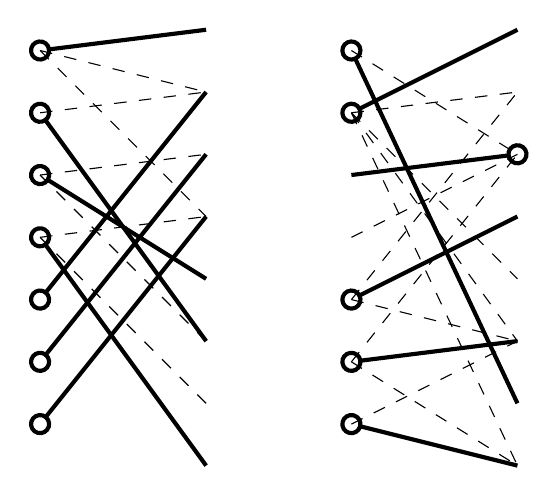
\begin{tikzpicture}[x=0.75pt,y=0.75pt,yscale=-1,xscale=1]
%uncomment if require: \path (0,341); %set diagram left start at 0, and has height of 341

%Straight Lines [id:da348664619914107] 
\draw [line width=1.5]    (73.33,39.58) -- (150,30) ;
\draw [shift={(70,40)}, rotate = 352.87] [color={rgb, 255:red, 0; green, 0; blue, 0 }  ][line width=1.5]      (0, 0) circle [x radius= 4.36, y radius= 4.36]   ;
%Straight Lines [id:da9283522339771824] 
\draw  [dash pattern={on 4.5pt off 4.5pt}]  (70,70) -- (150,60) ;
%Straight Lines [id:da9410354344174225] 
\draw  [dash pattern={on 4.5pt off 4.5pt}]  (70,40) -- (113.53,50.88) -- (150,60) ;
%Straight Lines [id:da7479833106357714] 
\draw  [dash pattern={on 4.5pt off 4.5pt}]  (70,130) -- (150,120) ;
%Straight Lines [id:da6512371495084972] 
\draw  [dash pattern={on 4.5pt off 4.5pt}]  (70,100) -- (150,90) ;
%Straight Lines [id:da6618764398559762] 
\draw  [dash pattern={on 4.5pt off 4.5pt}]  (70,40) -- (150,120) ;
%Straight Lines [id:da6556130949191818] 
\draw [line width=1.5]    (150,60) -- (72.1,157.38) ;
\draw [shift={(70,160)}, rotate = 128.66] [color={rgb, 255:red, 0; green, 0; blue, 0 }  ][line width=1.5]      (0, 0) circle [x radius= 4.36, y radius= 4.36]   ;
%Straight Lines [id:da2938319741216293] 
\draw [line width=1.5]    (150,90) -- (72.1,187.38) ;
\draw [shift={(70,190)}, rotate = 128.66] [color={rgb, 255:red, 0; green, 0; blue, 0 }  ][line width=1.5]      (0, 0) circle [x radius= 4.36, y radius= 4.36]   ;
%Straight Lines [id:da5461674454702563] 
\draw [line width=1.5]    (150,120) -- (72.1,217.38) ;
\draw [shift={(70,220)}, rotate = 128.66] [color={rgb, 255:red, 0; green, 0; blue, 0 }  ][line width=1.5]      (0, 0) circle [x radius= 4.36, y radius= 4.36]   ;
%Straight Lines [id:da6706884204764174] 
\draw [line width=1.5]    (150,150) -- (72.85,101.78) ;
\draw [shift={(70,100)}, rotate = 212.01] [color={rgb, 255:red, 0; green, 0; blue, 0 }  ][line width=1.5]      (0, 0) circle [x radius= 4.36, y radius= 4.36]   ;
%Straight Lines [id:da4349307802819935] 
\draw  [dash pattern={on 4.5pt off 4.5pt}]  (150,180) -- (70,100) ;
%Straight Lines [id:da6945730108329458] 
\draw [line width=1.5]    (150,180) -- (71.97,72.71) ;
\draw [shift={(70,70)}, rotate = 233.97] [color={rgb, 255:red, 0; green, 0; blue, 0 }  ][line width=1.5]      (0, 0) circle [x radius= 4.36, y radius= 4.36]   ;
%Straight Lines [id:da126152491590666] 
\draw [line width=1.5]    (150,240) -- (71.97,132.71) ;
\draw [shift={(70,130)}, rotate = 233.97] [color={rgb, 255:red, 0; green, 0; blue, 0 }  ][line width=1.5]      (0, 0) circle [x radius= 4.36, y radius= 4.36]   ;
%Straight Lines [id:da6810509862584775] 
\draw  [dash pattern={on 4.5pt off 4.5pt}]  (150,210) -- (70,130) ;
%Straight Lines [id:da5574395638694283] 
\draw  [dash pattern={on 4.5pt off 4.5pt}]  (220,70) -- (300,60) ;
%Straight Lines [id:da22811254014523996] 
\draw [line width=1.5]    (223,68.5) -- (300,30) ;
\draw [shift={(220,70)}, rotate = 333.43] [color={rgb, 255:red, 0; green, 0; blue, 0 }  ][line width=1.5]      (0, 0) circle [x radius= 4.36, y radius= 4.36]   ;
%Straight Lines [id:da5526258589996007] 
\draw  [dash pattern={on 4.5pt off 4.5pt}]  (220,40) -- (300,90) ;
%Straight Lines [id:da6365008691682541] 
\draw [line width=1.5]    (220,100) -- (296.67,90.42) ;
\draw [shift={(300,90)}, rotate = 352.87] [color={rgb, 255:red, 0; green, 0; blue, 0 }  ][line width=1.5]      (0, 0) circle [x radius= 4.36, y radius= 4.36]   ;
%Straight Lines [id:da734849273400068] 
\draw  [dash pattern={on 4.5pt off 4.5pt}]  (220,130) -- (300,90) ;
%Straight Lines [id:da6608002238859811] 
\draw  [dash pattern={on 4.5pt off 4.5pt}]  (220,160) -- (300,60) ;
%Straight Lines [id:da4204620259536589] 
\draw [line width=1.5]    (223,158.5) -- (300,120) ;
\draw [shift={(220,160)}, rotate = 333.43] [color={rgb, 255:red, 0; green, 0; blue, 0 }  ][line width=1.5]      (0, 0) circle [x radius= 4.36, y radius= 4.36]   ;
%Straight Lines [id:da6138234975700974] 
\draw  [dash pattern={on 4.5pt off 4.5pt}]  (220,70) -- (300,150) ;
%Straight Lines [id:da7174281483386467] 
\draw  [dash pattern={on 4.5pt off 4.5pt}]  (220,70) -- (300,180) ;
%Straight Lines [id:da7481175858554947] 
\draw  [dash pattern={on 4.5pt off 4.5pt}]  (220,70) -- (300,240) ;
%Straight Lines [id:da37186369112075357] 
\draw [line width=1.5]    (221.43,43.04) -- (300,210) ;
\draw [shift={(220,40)}, rotate = 64.8] [color={rgb, 255:red, 0; green, 0; blue, 0 }  ][line width=1.5]      (0, 0) circle [x radius= 4.36, y radius= 4.36]   ;
%Straight Lines [id:da5187871158245847] 
\draw  [dash pattern={on 4.5pt off 4.5pt}]  (220,190) -- (300,90) ;
%Straight Lines [id:da6327947654191872] 
\draw  [dash pattern={on 4.5pt off 4.5pt}]  (220,160) -- (300,180) ;
%Straight Lines [id:da8811792377084473] 
\draw [line width=1.5]    (223.33,189.58) -- (300,180) ;
\draw [shift={(220,190)}, rotate = 352.87] [color={rgb, 255:red, 0; green, 0; blue, 0 }  ][line width=1.5]      (0, 0) circle [x radius= 4.36, y radius= 4.36]   ;
%Straight Lines [id:da9895881120708945] 
\draw  [dash pattern={on 4.5pt off 4.5pt}]  (220,190) -- (300,240) ;
%Straight Lines [id:da20793919100446723] 
\draw [line width=1.5]    (223.25,220.81) -- (300,240) ;
\draw [shift={(220,220)}, rotate = 14.04] [color={rgb, 255:red, 0; green, 0; blue, 0 }  ][line width=1.5]      (0, 0) circle [x radius= 4.36, y radius= 4.36]   ;
%Straight Lines [id:da8522182769629001] 
\draw  [dash pattern={on 4.5pt off 4.5pt}]  (220,220) -- (300,180) ;
\end{tikzpicture}
\end{figure*}

The matching is represented by bolded edges and corresponding cover vertices are denoted with open circles $\Box$

\end{document}

% List of tex snippets:
%   - tex-header (this)
%   - R      --> \mathbb{R}
%   - Z      --> \mathbb{Z}
%   - B      --> \mathcal{B}
%   - E      --> \mathcal{E}
%   - M      --> \mathcal{M}
%   - m      --> \mathfrak{m}({#1})
%   - normlp --> \norm{{#1}}_{L^{{#2}}}
